\section{Discovered objects}

It was not until 2017 when the first interstellar object was discovered. The
object, initially named 1I/2017 U1, is known today as 1I/'Oumuamua. Two years
later, in 2019, the second interstellar object was discovered. The object was
beleived to be a comet and was named C/2019 Q4. After confirming its ISO nature,
today the object is know as 2I/Borisov. 

Despite having a common interstellar origin, both objects presented different
properties. These properties are presented and discussed in the following
subsections. For a more detailed analysis of the objects and their properties,
the reader is encouraged to review the article by \cite{jewitt2023}.

\subsection{1I/'Oumuamua}

'Oumuamua was discovered on October 19, 2017, by the Pan-STARRS1 telescope in
Hawaii. It was first classified as a comet under the identifier of C/2017 U1,
but later reclassified as an an asteroid.

Its eccentricity was calculated to be around $1.20$, thus showing an hyperbolic
orbit. Its velocity was calculated to be close to $26.0$ km/s. Finally, it
entered the solar system with a direction $\alpha_{\text{ICRS}},\;
\delta_{\text{ICRS}} = 279^\circ.804,\; +33^\circ.997$, an inclination far from
the invariant plane of the solar system and close to the solar apex, see
\cite{mamajek2017}. All these attributes are consistent with an interstellar
origin, as exposed in subsection \ref{sec:expected_orbit_attributes}. Table 

\begin{table}[H]
  \centering
  \begin{tabular}{|c|c|}
    \hline
    Element & Value \\
    \hline
    Eccentricity ($e$) & 1.20 \\
    Semi-major axis ($a$) & -1.27 au \\
    Perihelion ($q$) & 0.26 au \\
    Inclination ($i$) & 122.74 deg \\
    Longitude of the ascending node ($\Omega$) & 24.59 deg \\
    Argument of perihelion ($\omega$) & 241.81 deg \\
    Mean anomaly ($M$) & 51.16 deg \\
    Mean motion ($n$) & 0.69 deg/d \\
    Time of perihelion passage ($T_p$) & 2017-Nov-23 \\
    \hline
  \end{tabular}
  \caption{Orbit elements of 1I/'Oumuamua as provided by the NASA SBDB.}
  \label{tab:oumuamua_elements}
\end{table}

Surprisingly, this first discovered ISO presented a non-gravitational
acceleration that could not be attributed to cometary properties. In addition,
observations could not determine jetting of particles, an effect experienced by
cometary objects.

'Oumuamua's shape was also a matter of debate. Due to its size, the interloper
appeared as a single point in all telescope images, like the one reproduced in
figure \ref{fig:oumuamua_shape}. At first, it was estimated to have a cigar-like
body. However, later studies solved the best fititng shape that matched the
observed lightcurves. The results indicate that 'Oumuamua should have a planar
disk shape, see \cite{seligman2022}. Unfortunately, 'Oumuamua was discovered
after its pasage through the perihelion and could only be observed for about
four weeks before becoming to faint. This limited the amount of data that could
be gathered about the object, increasing the mistery about the first
interstellar object.


\subsection{2I/Borisov}

Borisov was discovered on August 30, 2019, by Gennady Borisov\footnote{Borisov
discovered the second interloper using his home-built 0.65 meters
telescope.}, an amateur astronomer from Crimea. It was first classified as
a comet under the identifier C/2019 Q4, but later reclassified as an
interstellar object once its high eccentricity was computed.

With an eccentricity of $3.36$, it showed a hyperbolic orbit with a velocity of
$32.2$ km/s. With an inclination of $44.1$ in addition to all previous
properties, it was evident that Borisov came from outside the solar system.

The main difference with 'Ouamuamua was that Borisov showed a cometary tail. In
fact, the NASA/ESA Hubble Space Telescope was able to capture some images of
this ISO


\newpage

\begin{figure}[H]
  \centering
  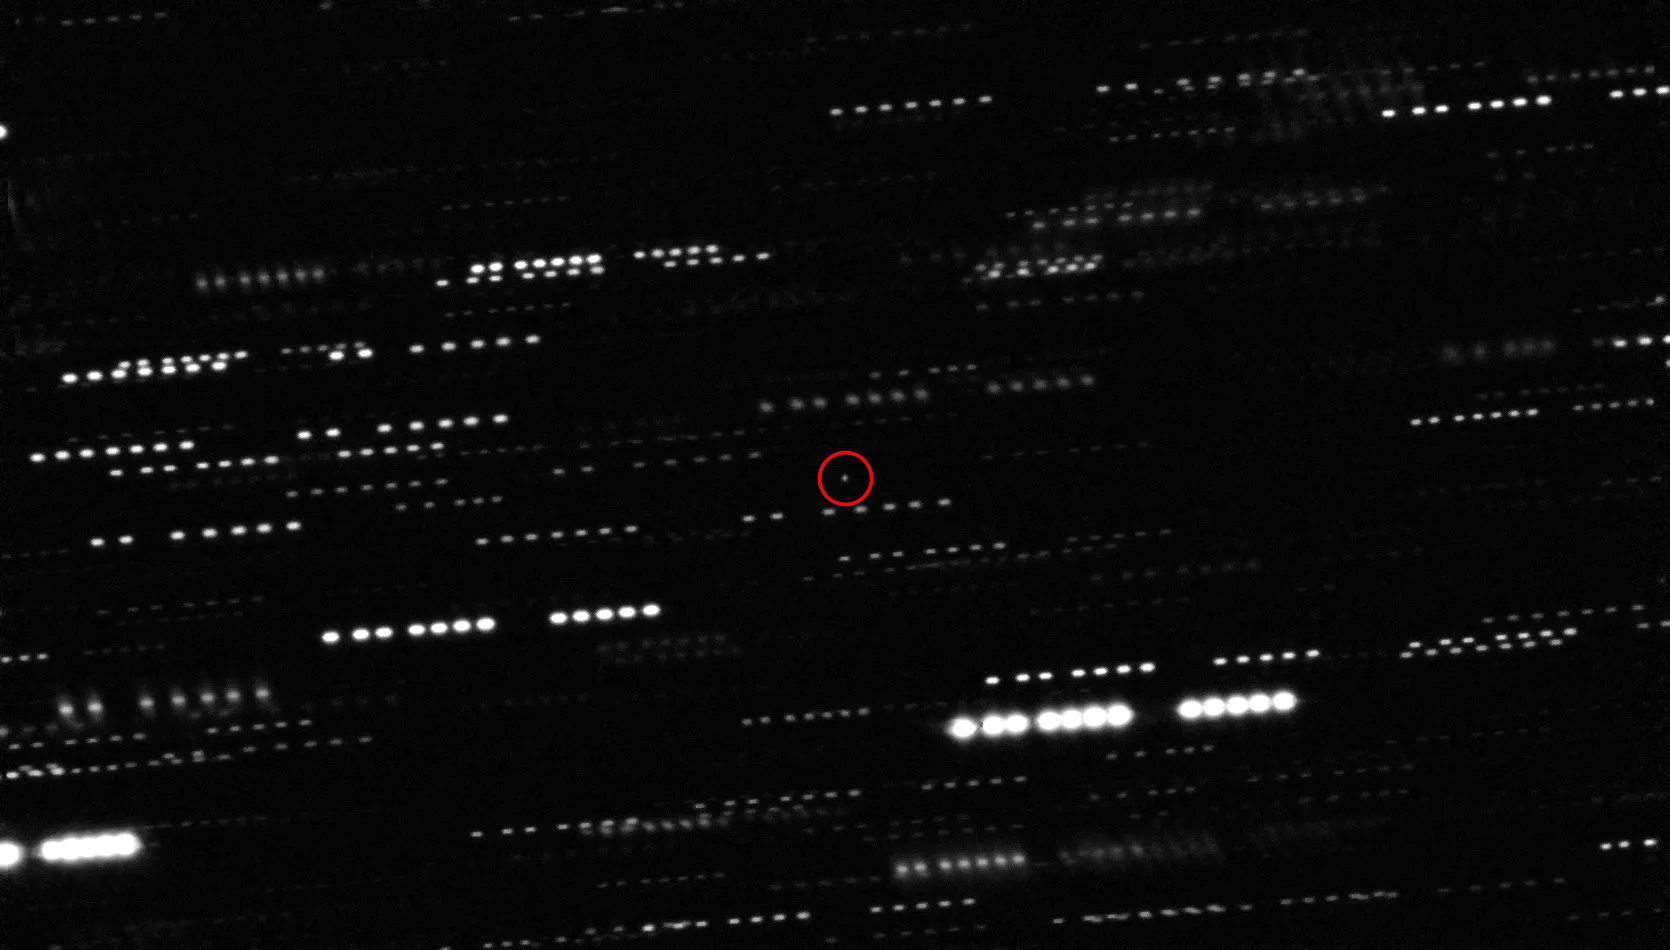
\includegraphics[width=0.95\textwidth]{static/oumuamua/shape.png}
\caption['Oumuamua as seen by the ESO's Very Large Telescope and the Gemini South Telescope]{
  1I/'Oumuamua as seen by the ESO's Very Large Telescope and the Gemini South Telescope. This image was
  released on September 9, 2023. It shows a combination of images taken by the two
  telecopes. The object is seen as a point in the center of the image. Background
  stars are seen as streaks due to the telescope's tracking of the object. No
  cometary tail or mass ejection is observed, raising questions about the non-gravitational
  acceleration presented by the interloper.
  }
  \label{fig:oumuamua_shape}
\end{figure}

\begin{figure}[H]
  \centering
  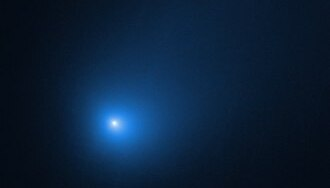
\includegraphics[width=0.95\textwidth]{static/borisov/shape.jpg}
\caption[Borisov as seen by the NASA/ESA Hubble Space Telescope]{
  2I/Borisov as seen by the NASA/ESA Hubble Space Telescope. This image was
  released on December 12, 2019, when the interloper was close to the Sun. Its
  cometary properties are evident in this image. Borisov's tail is seen as a
faint streak extending from the object. It is believed that the tail is composed
of 
  }
  \label{fig:borisov_shape}
\end{figure}







%
%...
%
%
%\subsection{Other candidates}
%
%...
